\begin{activity} \label{A:3.2.3} 
 Let $\ds L(t) = \frac{A}{1+ce^{-kt}}$, where $A$, $c$, and $k$ are all positive real numbers.
	 \ba
		\item Observe that we can equivalently write $L(t) = A(1+ce^{-kt})^{-1}$.  Find $L'(t)$ and explain why $L$ has no critical values.  Is $L$ always increasing or always decreasing?  Why?
	 	\item Given the fact that
		$$L''(t) = Ack^2e^{-kt} \frac{ce^{-kt}-1}{(1+ce^{-kt})^3},$$
		find all values of $t$ such that $L''(t) = 0$ and hence construct a second derivative sign chart.  For which values of $t$ is a function in this family concave up?  concave down?
		\item What is the value of $\ds \lim_{t \to \infty} \frac{A}{1+ce^{-kt}}$? $\ds \lim_{t \to -\infty} \frac{A}{1+ce^{-kt}}$?
		\item Find the value of $L(x)$ at the inflection point found in (b).
	  	\item Without using a graphing utility, sketch the graph of a typical member of this family. Write several sentences to describe the overall behavior of a typical function $h$ and how this behavior depends on $a$ and $b$.
		\item Explain why it is reasonable to think that the function $L(t)$ models the growth of a population over time in a setting where the largest possible population the surrounding environment can support is $A$.
	 \ea
\end{activity}
\begin{smallhint}
	 \ba
		\item Use the chain rule, treating $A$, $c$, and $k$ as constants.
	 	\item Note that the only way $L''(t) = 0$ is if $ce^{-kt}-1 = 0$.
		\item Remember that $e^{-t} \to 0$ as $t \to \infty$ and $e^{-t} \to \infty$ as $t \to -\infty$.
		\item Don't forget that $e^{\ln(x)} = x$ for all $x > 0$.
	  	\item Think about horizontal asymptotes, where $L$ is increasing and decreasing, and concavity.
	 \ea
\end{smallhint}
\begin{bighint}
	 \ba
		\item Use the chain rule, treating $A$, $c$, and $k$ as constants.  Remember that $e^{-kt} > 0$ for all values of $t$.
	 	\item Note that the only way $L''(t) = 0$ is if $ce^{-kt}-1 = 0$.  Observe that since $ce^{-kt} \to 0$ as $t \to \infty$, the quantity $ce^{-kt} - 1$ will be positive to the left of where it is zero and negative to the right of where it is zero.
		\item Remember that $e^{-t} \to 0$ as $t \to \infty$ and $e^{-t} \to \infty$ as $t \to -\infty$.
		\item Don't forget that $e^{\ln(x)} = x$ for all $x > 0$.
	  	\item Think about horizontal asymptotes, where $L$ is increasing and decreasing, and concavity.  In addition, find $L(0)$ and plot both this point and the inflection point.
	 \ea
\end{bighint}
\begin{activitySolution}
	 \ba
		\item By the chain rule and treating $A$, $c$, and $k$ as constants, we find that
		$$L'(t) = A(-1)(1+ce^{-kt})^{-2} ce^{-kt}(-k) = Acke^{-kt}(1+ce^{-kt})^{-2}.$$  
		Since $A$, $c$, and $k$ are all positive and $e^{-kt} > 0$ for all values of $t$, it is apparent that $L'(t)$ is never zero, and indeed is positive for every value of $t$.  Thus, $L$ is an always increasing function.
	 	\item  Given that
		$$L''(t) = Ack^2e^{-kt} \frac{ce^{-kt}-1}{(1+ce^{-kt})^3},$$ the only way $L''(t) = 0$ is if $ce^{-kt}-1 = 0$.  Solving $ce^{-kt}-1 = 0$ for $t$, we first write $e^{-kt} = \frac{1}{c}$.  Taking the natural logarithm of both sides, $-kt = \ln(\frac{1}{c})$, so that
		$$t = -\frac{1}{k} \ln \left(\frac{1}{c}\right)$$
		is the only value of $t$ for which $L''(t) = 0$.  Now, observe that since $ce^{-kt} \to 0$ as $t \to \infty$, the quantity $ce^{-kt} - 1$ will be positive to the left of where it is zero and negative to the right of where it is zero.  Since this is the only term in $L''(t)$ that can change sign, it follows that $L''(t) > 0$ for $t < -\frac{1}{k} \ln \left(\frac{1}{c}\right)$ and $L''(t) > 0$ for $t > -\frac{1}{k} \ln \left(\frac{1}{c}\right)$, making $L$ concave up to the left of the noted inflection point and concave down thereafter.
		\item Recalling that $e^{-kt} \to 0$ as $t \to \infty$, we observe that
		 $$\lim_{t \to \infty} \frac{A}{1+ce^{-kt}} = \frac{A}{1+0} = A,$$
		 so $L$ has a horizontal asymptote of $y = A$ as $t \to \infty$.  On the other hand, since $e^{-kt} \to \infty$ as $t \to -\infty$, this causes the denominator of $L$ to grow without bound (while the numerator remains constant), and therefore
		 		 $$\lim_{t \to \infty} \frac{A}{1+ce^{-kt}} = 0,$$
				 which means $L$ has a horizontal asymptote of $y = 0$ as $t \to -\infty$.
		\item From (b), we know that $t = -\frac{1}{k} \ln \left(\frac{1}{c}\right)$ is the location of the inflection point of $L$.  Evaluating the function at this point, we find that
		$$L\left( -\frac{1}{k} \ln \left(\frac{1}{c}\right) \right) = \frac{A}{1+ce^{-k [-\frac{1}{k} \ln \left(\frac{1}{c}\right)]}} = \frac{A}{1+ce^{\ln \left(\frac{1}{c}\right)}} = \frac{A}{1+c \cdot \frac{1}{c}} = \frac{A}{2}.$$
		Thus, the inflection point on the graph of $L$ is located at  $( -\frac{1}{k} \ln \left(\frac{1}{c}\right), \frac{A}{2})$.
	  	\item We have shown that $L$ is an always increasing function that has horizontal asymptotes at $y =0$ and $y = A$, as well as an inflection point at $( -\frac{1}{k} \ln \left(\frac{1}{c}\right), \frac{A}{2})$, which we note lies vertically halfway between the asymptotes.  In addition, we see that $L(0) = \frac{A}{1+c}$.  The combination of all of this information shows us that a typical graph in this family of functions is given by the following figure.
  \begin{center}
  	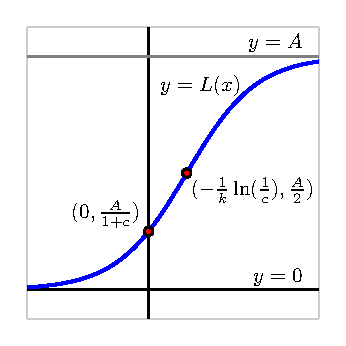
\includegraphics{figures/3_2_Act3Soln.eps}
  \end{center}
	 \ea
\end{activitySolution}
\aftera
















